\documentclass{standalone}
\usepackage{tikz}
\usetikzlibrary{patterns, positioning}

\begin{document}
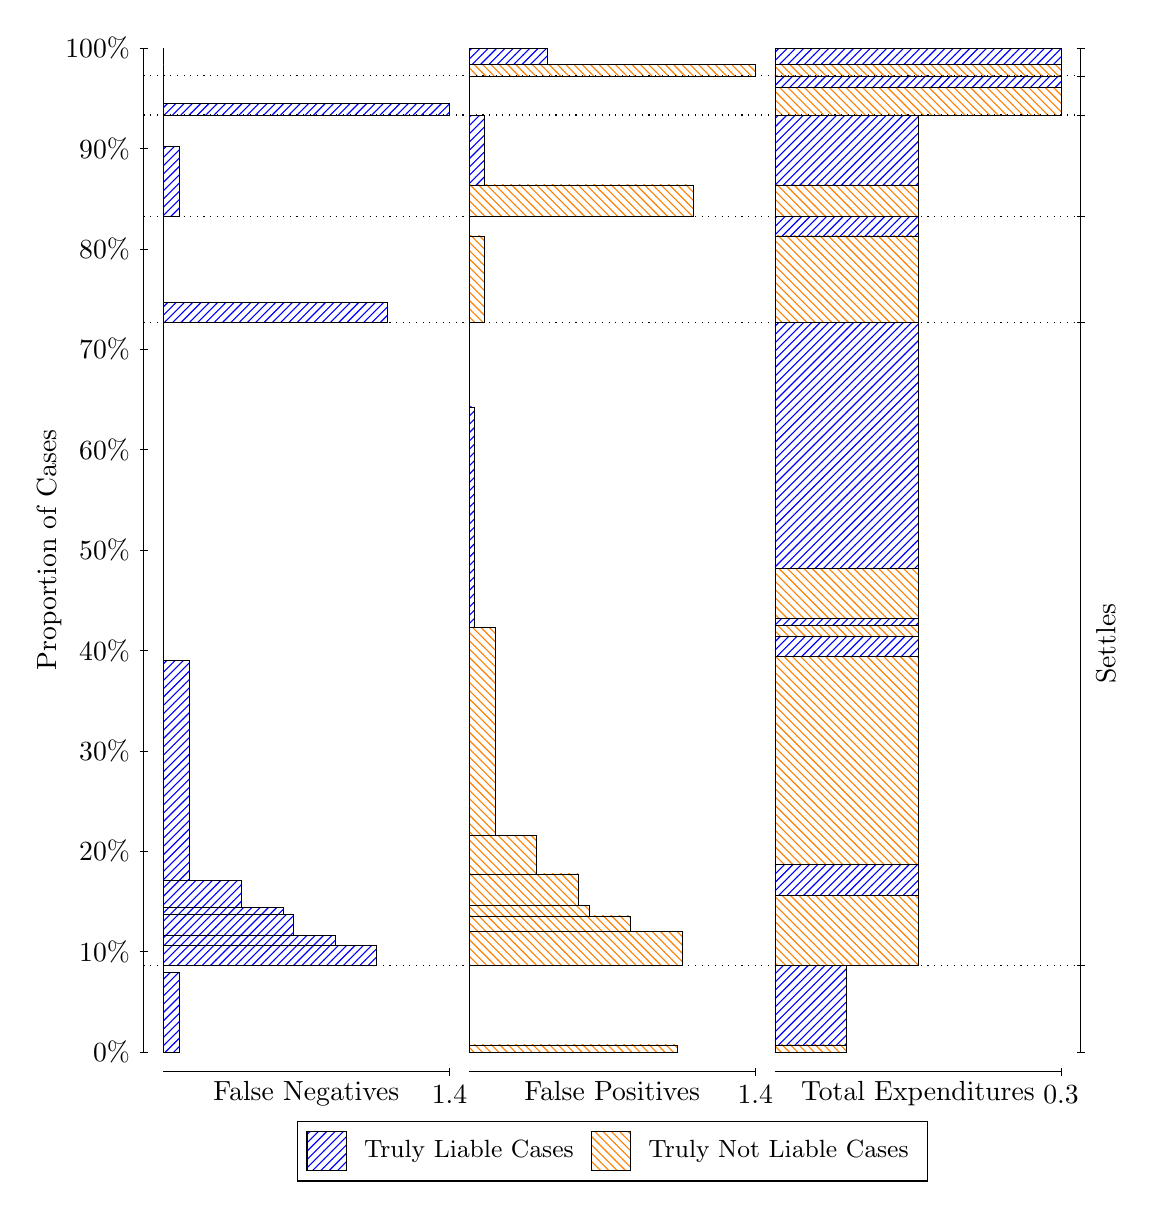
\begin{tikzpicture}
\draw[black, very thin] (1.5,1.75) -- (1.5,14.5);
\node[rotate=90, anchor=center] at (0.3, 8.125) {Proportion of Cases};
\draw[black, very thin] (1.45,1.75) -- (1.55,1.75);
\node[anchor=east] at (1.45, 1.75) {0\%};
\draw[black, very thin] (1.45,3.025) -- (1.55,3.025);
\node[anchor=east] at (1.45, 3.025) {10\%};
\draw[black, very thin] (1.45,4.3) -- (1.55,4.3);
\node[anchor=east] at (1.45, 4.3) {20\%};
\draw[black, very thin] (1.45,5.575) -- (1.55,5.575);
\node[anchor=east] at (1.45, 5.575) {30\%};
\draw[black, very thin] (1.45,6.85) -- (1.55,6.85);
\node[anchor=east] at (1.45, 6.85) {40\%};
\draw[black, very thin] (1.45,8.125) -- (1.55,8.125);
\node[anchor=east] at (1.45, 8.125) {50\%};
\draw[black, very thin] (1.45,9.4) -- (1.55,9.4);
\node[anchor=east] at (1.45, 9.4) {60\%};
\draw[black, very thin] (1.45,10.675) -- (1.55,10.675);
\node[anchor=east] at (1.45, 10.675) {70\%};
\draw[black, very thin] (1.45,11.95) -- (1.55,11.95);
\node[anchor=east] at (1.45, 11.95) {80\%};
\draw[black, very thin] (1.45,13.225) -- (1.55,13.225);
\node[anchor=east] at (1.45, 13.225) {90\%};
\draw[black, very thin] (1.45,14.5) -- (1.55,14.5);
\node[anchor=east] at (1.45, 14.5) {100\%};

\draw[black, very thin] (13.4,1.75) -- (13.4,14.5);
\draw[black, very thin] (13.35,1.75) -- (13.45,1.75);
\node[anchor=west] at (13.35, 1.75) {};
\draw[black, very thin] (13.35,2.8497) -- (13.45,2.8497);
\node[anchor=west] at (13.35, 2.8497) {};
\draw[black, very thin] (13.35,11.019) -- (13.45,11.019);
\node[anchor=west] at (13.35, 11.019) {};
\draw[black, very thin] (13.35,12.365) -- (13.45,12.365);
\node[anchor=west] at (13.35, 12.365) {};
\draw[black, very thin] (13.35,13.649) -- (13.45,13.649);
\node[anchor=west] at (13.35, 13.649) {};
\draw[black, very thin] (13.35,14.146) -- (13.45,14.146);
\node[anchor=west] at (13.35, 14.146) {};
\draw[black, very thin] (13.35,14.5) -- (13.45,14.5);
\node[anchor=west] at (13.35, 14.5) {};

\draw[black, very thin, pattern color=blue, pattern=north east lines] (1.75,1.75) rectangle (1.9482,2.7607);
\draw[black, very thin, pattern color=orange, pattern=north west lines] (1.75,2.7607) rectangle (1.75,2.8497);
\draw[black, very thin, pattern color=blue, pattern=north east lines] (1.75,2.8497) rectangle (4.4585,3.1014);
\draw[black, very thin, pattern color=blue, pattern=north east lines] (1.75,3.1014) rectangle (3.93,3.2329);
\draw[black, very thin, pattern color=blue, pattern=north east lines] (1.75,3.2329) rectangle (3.4015,3.4978);
\draw[black, very thin, pattern color=blue, pattern=north east lines] (1.75,3.4978) rectangle (3.2694,3.5899);
\draw[black, very thin, pattern color=blue, pattern=north east lines] (1.75,3.5899) rectangle (2.7409,3.9269);
\draw[black, very thin, pattern color=blue, pattern=north east lines] (1.75,3.9269) rectangle (2.0803,6.7219);
\draw[black, very thin, pattern color=orange, pattern=north west lines] (1.75,6.7219) rectangle (1.75,11.019);
\draw[black, very thin, pattern color=blue, pattern=north east lines] (1.75,11.019) rectangle (4.5906,11.269);
\draw[black, very thin, pattern color=orange, pattern=north west lines] (1.75,11.269) rectangle (1.75,12.365);
\draw[black, very thin, pattern color=blue, pattern=north east lines] (1.75,12.365) rectangle (1.9482,13.253);
\draw[black, very thin, pattern color=orange, pattern=north west lines] (1.75,13.253) rectangle (1.75,13.649);
\draw[black, very thin, pattern color=blue, pattern=north east lines] (1.75,13.649) rectangle (5.3833,13.792);
\draw[black, very thin, pattern color=orange, pattern=north west lines] (1.75,13.792) rectangle (1.75,14.146);
\draw[black, very thin, pattern color=orange, pattern=north west lines] (1.75,14.146) rectangle (1.75,14.289);
\draw[black, very thin, pattern color=blue, pattern=north east lines] (1.75,14.289) rectangle (1.75,14.5);
\draw[black, very thin, pattern color=orange, pattern=north west lines] (5.6333,1.75) rectangle (8.2758,1.839);
\draw[black, very thin, pattern color=blue, pattern=north east lines] (5.6333,1.839) rectangle (5.6333,2.8497);
\draw[black, very thin, pattern color=orange, pattern=north west lines] (5.6333,2.8497) rectangle (8.3418,3.2812);
\draw[black, very thin, pattern color=orange, pattern=north west lines] (5.6333,3.2812) rectangle (7.6812,3.4787);
\draw[black, very thin, pattern color=orange, pattern=north west lines] (5.6333,3.4787) rectangle (7.1527,3.6161);
\draw[black, very thin, pattern color=orange, pattern=north west lines] (5.6333,3.6161) rectangle (7.0206,4.0116);
\draw[black, very thin, pattern color=orange, pattern=north west lines] (5.6333,4.0116) rectangle (6.4921,4.5043);
\draw[black, very thin, pattern color=orange, pattern=north west lines] (5.6333,4.5043) rectangle (5.9636,7.1467);
\draw[black, very thin, pattern color=blue, pattern=north east lines] (5.6333,7.1467) rectangle (5.6994,9.9417);
\draw[black, very thin, pattern color=blue, pattern=north east lines] (5.6333,9.9417) rectangle (5.6333,11.019);
\draw[black, very thin, pattern color=orange, pattern=north west lines] (5.6333,11.019) rectangle (5.8315,12.115);
\draw[black, very thin, pattern color=blue, pattern=north east lines] (5.6333,12.115) rectangle (5.6333,12.365);
\draw[black, very thin, pattern color=orange, pattern=north west lines] (5.6333,12.365) rectangle (8.4739,12.761);
\draw[black, very thin, pattern color=blue, pattern=north east lines] (5.6333,12.761) rectangle (5.8315,13.649);
\draw[black, very thin, pattern color=orange, pattern=north west lines] (5.6333,13.649) rectangle (5.6333,14.003);
\draw[black, very thin, pattern color=blue, pattern=north east lines] (5.6333,14.003) rectangle (5.6333,14.146);
\draw[black, very thin, pattern color=orange, pattern=north west lines] (5.6333,14.146) rectangle (9.2667,14.289);
\draw[black, very thin, pattern color=blue, pattern=north east lines] (5.6333,14.289) rectangle (6.6242,14.5);
\draw[black, very thin, pattern color=orange, pattern=north west lines] (9.5167,1.75) rectangle (10.425,1.839);
\draw[black, very thin, pattern color=blue, pattern=north east lines] (9.5167,1.839) rectangle (10.425,2.8497);
\draw[black, very thin, pattern color=orange, pattern=north west lines] (9.5167,2.8497) rectangle (11.333,3.738);
\draw[black, very thin, pattern color=blue, pattern=north east lines] (9.5167,3.738) rectangle (11.333,4.1343);
\draw[black, very thin, pattern color=orange, pattern=north west lines] (9.5167,4.1343) rectangle (11.333,6.7767);
\draw[black, very thin, pattern color=blue, pattern=north east lines] (9.5167,6.7767) rectangle (11.333,7.0283);
\draw[black, very thin, pattern color=orange, pattern=north west lines] (9.5167,7.0283) rectangle (11.333,7.1658);
\draw[black, very thin, pattern color=blue, pattern=north east lines] (9.5167,7.1658) rectangle (11.333,7.2579);
\draw[black, very thin, pattern color=orange, pattern=north west lines] (9.5167,7.2579) rectangle (11.333,7.8868);
\draw[black, very thin, pattern color=blue, pattern=north east lines] (9.5167,7.8868) rectangle (11.333,11.019);
\draw[black, very thin, pattern color=orange, pattern=north west lines] (9.5167,11.019) rectangle (11.333,12.115);
\draw[black, very thin, pattern color=blue, pattern=north east lines] (9.5167,12.115) rectangle (11.333,12.365);
\draw[black, very thin, pattern color=orange, pattern=north west lines] (9.5167,12.365) rectangle (11.333,12.761);
\draw[black, very thin, pattern color=blue, pattern=north east lines] (9.5167,12.761) rectangle (11.333,13.649);
\draw[black, very thin, pattern color=orange, pattern=north west lines] (9.5167,13.649) rectangle (13.15,14.003);
\draw[black, very thin, pattern color=blue, pattern=north east lines] (9.5167,14.003) rectangle (13.15,14.146);
\draw[black, very thin, pattern color=orange, pattern=north west lines] (9.5167,14.146) rectangle (13.15,14.289);
\draw[black, very thin, pattern color=blue, pattern=north east lines] (9.5167,14.289) rectangle (13.15,14.5);
\draw[black, dotted] (1.5,2.8497) -- (13.4,2.8497);
\draw[black, dotted] (1.5,11.019) -- (13.4,11.019);
\draw[black, dotted] (1.5,12.365) -- (13.4,12.365);
\draw[black, dotted] (1.5,13.649) -- (13.4,13.649);
\draw[black, dotted] (1.5,14.146) -- (13.4,14.146);
\draw[black, very thin] (1.75,1.5) -- (5.3833,1.5);
\node[anchor=north] at (3.5667, 1.5) {False Negatives};
\draw[black, very thin] (5.3833,1.45) -- (5.3833,1.55);
\node[anchor=north] at (5.3833, 1.45) {1.4};

\draw[black, very thin] (5.6333,1.5) -- (9.2667,1.5);
\node[anchor=north] at (7.45, 1.5) {False Positives};
\draw[black, very thin] (9.2667,1.45) -- (9.2667,1.55);
\node[anchor=north] at (9.2667, 1.45) {1.4};

\draw[black, very thin] (9.5167,1.5) -- (13.15,1.5);
\node[anchor=north] at (11.333, 1.5) {Total Expenditures};
\draw[black, very thin] (13.15,1.45) -- (13.15,1.55);
\node[anchor=north] at (13.15, 1.45) {0.3};


\node[black, centered, rotate=90] at (13.72, 6.9343) {Settles};





\draw (7.449999999999999,1.5) node[draw=none] (baseCoordinate) {};
\begin{scope}[align=center]
        \matrix[scale=0.5, draw=black, below=0.5cm of baseCoordinate, nodes={draw}, column sep=0.1cm]{
            \node[rectangle, draw, minimum width=0.5cm, minimum height=0.5cm, pattern=north east lines, pattern color=blue] {}; &
            \node[draw=none, font=\small] (B) {Truly Liable Cases}; &
            \node[rectangle, draw, minimum width=0.5cm, minimum height=0.5cm, pattern=north west lines, pattern color=orange] {}; &
            \node[draw=none, font=\small] (B) {Truly Not Liable Cases}; \\
            };
\end{scope}

\end{tikzpicture}
\end{document}